% !TEX TS-program = XeLaTeX
% Commands for running this example:
% 	 xelatex wrapfig
% End of Commands
\documentclass[a4paper,12pt]{article}
\pagestyle{empty}
\usepackage{graphicx}
\usepackage{wrapfig}
\usepackage[Kashida]{xepersian}

\begin{document}
جمشید بن مسعود بن محمود طبیب کاشانی ملقب به غیاث‌الدین که در غرب به الکاشی \lr{(Al-Kashi)} مشهور است. ریاضی‌دانی برجسته و ستاره‌شناس و محاسبی ماهر و زبردست بود. آلات رصدی دقیقی اختراع کرد و از حدود ۸۰۸ (۱۴۰۶) تا پایان عمرش ۸۳۲ (۱۴۲۹) فعالیت علمی داشته است. در دوران فعالیت علمی‌اش به تالیف کتاب‌های متعددی در زمینه ریاضیات و نجوم پرداخته است مهم‌ترین این آثار عبارت‌اند از: زیج خاقانی، مفتاح الحساب، رسالهٔ محیطیه و رسالهٔ وتر و جیب.

\begin{wrapfigure}{r}{0.5\textwidth}
  \begin{center}
    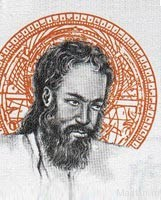
\includegraphics[width=0.48\textwidth]{ghjk}
  \end{center}
  \caption{غیاث‌الدین جمشید کاشانی (حدود ۷۹۰-۸۳۲) ریاضی‌دان و اخترشناس ایرانی}
\end{wrapfigure}

غیاث‌الدین جمشید کاشانی هر چند فیزیکدان بود، ولی علاقهٔ اصلی‌اش متوجه ریاضیات و اخترشناسی بود؛ پس از دورهٔ طولانی بی‌نوایی و سرگردانی، سرانجام در سایهٔ حمایت سلطان الغ‌بیگ، که خود دانشمند بزرگی بود، موقعیت شغلی مطمئنی در سمرقند به‌دست آورد.

غیاث‌الدین جمشید کاشانی، زبردست‌ترین حساب‌دان و آخرین ریاضی‌دان برجستهٔ دورهٔ اسلامی و از بزرگ‌ترین مفاخر تاریخ ایران به شمار می‌آید. وی به تکمیل وتصحیح روش‌های قدیمی انجام چهار عمل اصلی حساب پرداخت و روش‌های جدید و ساده‌تری برای آن‌ها اختراع کرد. در واقع، کاشانی را باید مخترع روش‌های کنونی انجام چهار عمل اصلی حساب (به ویژه ضرب و تقسیم) دانست. کتاب ارزشمند وی با نام مفتاح الحساب کتابی درسی، دربارهٔ ریاضیات مقدماتی است و آن را از حیث فراوانی و تنوع مواد و مطالب و روانی بیان سرآمد همهٔ آثار ریاضی سده‌های میانه می‌دانند.

ابداع و ترویج کسرهای اعشاری به قیاس با کسرهای شصتگانی که در ستاره‌شناسی متداول بود. محاسبهٔ عدد پی تا شانزده رقم اعشار به نحوی که تا صد و پنجاه سال بعد کسی نتوانست آن را گسترش دهد:  $2\pi=6.2831853071795865$.

محاسبه سینوس (جیب) زاویهٔ یک درجه با روش ابتکاری حل یک معادلهٔ درجه سوم: $\sin 1^\circ=0.0174524064372835103712$ هفده رقم اعشاری عدد به دست آمده با مقداری که امروزه محاسبه می‌شود هم خوانی دارد. در واقع کاشانی مقدار سینوس یک درجه را تا ده رقم صحیح شصتگانی حساب کرد.

اختراع ابزار اخترشناسی دقیق از جمله وسیله‌ای به نام «طبق المناطق» برای محاسب طول ستارگان که کتاب نزهت‌الحدائق در شرح آن است.

\end{document}
